%%%%%%%%%%%%%%%%%%%%%%%%%%%%%%%%%%%%%%%%%%%%%%%%%%%%%%%%%%%%%%%%%%%%
\section{Design} %(10 pages)
\label{sec:fdsp-apa-design}


%%%%%%%%%%%%%%%
\subsection{The DUNE Anode Plane Assemblies}
%\subsection{APA Overview, Key Design Parameters and Requirements}

The physics performance of the DUNE single-phase (SP) Far Detector is a function of many intertwined detector parameters including argon purity, drift distance, electric field, wire pitch, wire length, and noise levels in the readout electronics.  Energy deposits from minimum ionizing particles originating anywhere inside the active volume of the detector need to generate hits with signal-to-noise $>$ 9:1 in order to be reconstructed with $\approx 100\%$ efficiency.  These requirements set constraints on the APA design, such as limits on the wire pitch, wire length, choice of wire material.  In this section, we present an overview of the key parameters of the DUNE-SP APA design. 

The APA support frames are made from stainless steel hollow tube sections that are precision machined and bolted together. A fine, conducting mesh covers the rectangular openings in the frame, on both sides, to define a uniform ground plane across the frame. Along the length of the frame and around it, over the mesh layer, layers of sense and shielding wires are strung or wrapped at varying angles relative to each other. The wires are terminated on boards that anchor them and also provide the connections to the readout electronics. 

\begin{dunefigure}[APA diagram]{fig:apa-photo}
{ProtoDUNE APA. REPLACE WITH PHOTO OF FINISHED APA}
\setlength{\fboxsep}{0pt}
\setlength{\fboxrule}{0.5pt}
\fbox{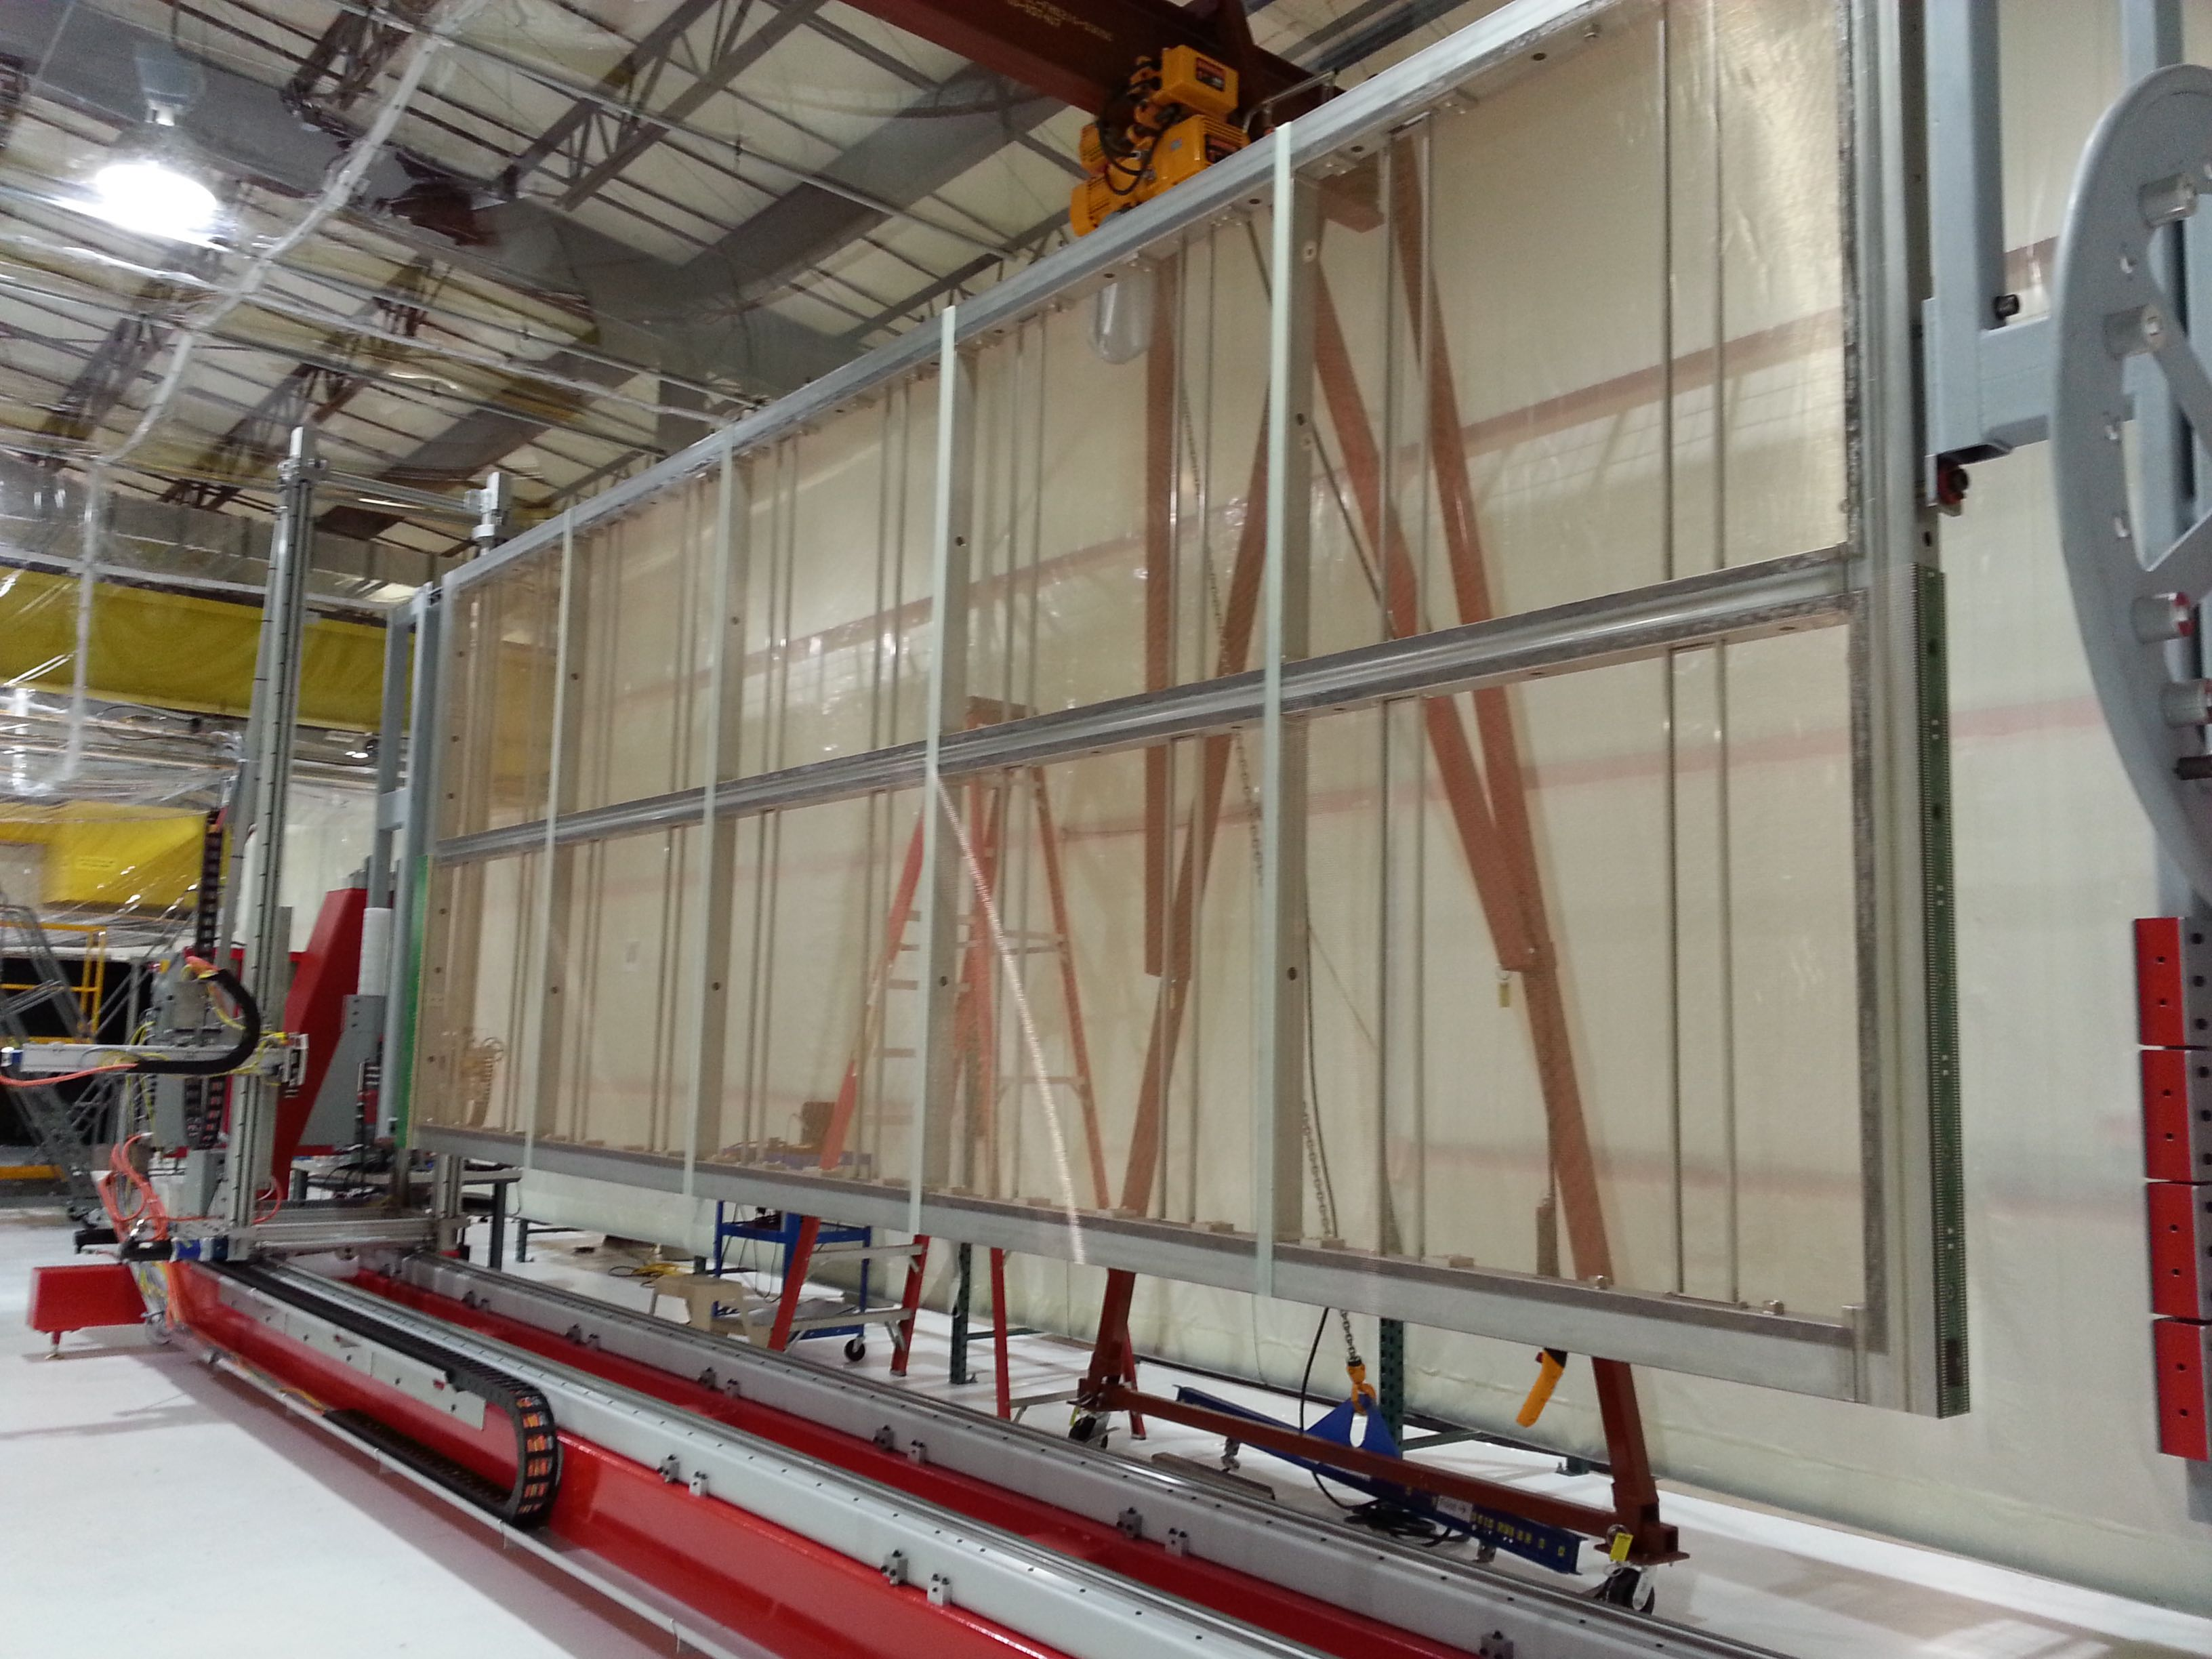
\includegraphics[width=0.95\textwidth,trim=0mm 100mm 0mm 0mm,clip]{APA-photo-on-winder.jpg}} 
\end{dunefigure}

In the current design of the DUNE-SP far detector module, a central row of APAs is flanked by drift-field regions on either side, requiring sensitivity on both sides. The wrapped APAs allow the induction plane wires to sense drifting ionization originating from either side of the APA.  This double-sided feature is also advantageous for the APAs located against the cryostat walls with a drift field on one side only, since the grid layer facing the wall effectively blocks any ionization generated outside the TPC from drifting in to the wires on that side of the APA.  

The APAs are approximately \SI{6}{m} high, \SI{2.3}{m} wide, and \SI{12}{cm} thick, with 4 layers of wires on each APA.  Figure~\ref{fig:apa-photo} shows one of the prototype APAs built for ProtoDUNE. Starting from the outermost wire layer, there is first an uninstrumented shielding plane (vertical), followed by two induction planes ($\pm 35.7^{\circ}$ to the vertical), and finally the collection plane (vertical). All wire layers span the entire height of the APA frame. The two planes of induction wires ($U$ and $V$) wrap in a helical fashion around the long edge, continuously around both sides of the APA. The layout of the wire layers is illustrated in Figure~\ref{fig:tpc_apa1}.  


\begin{dunefigure}[APA diagram]{fig:tpc_apa1}
{Illustration of the APA wire wrapping scheme. Small portions of the wires from the three signal planes are shown in color: magenta ($U$), green ($V$), blue ($X$). The fourth wire plane ($G$) above these three, parallel with $X$, is present to improve the pulse shape on the $U$ plane signals.} % (Right) Field lines and signal shapes on the induction and collection wires.}
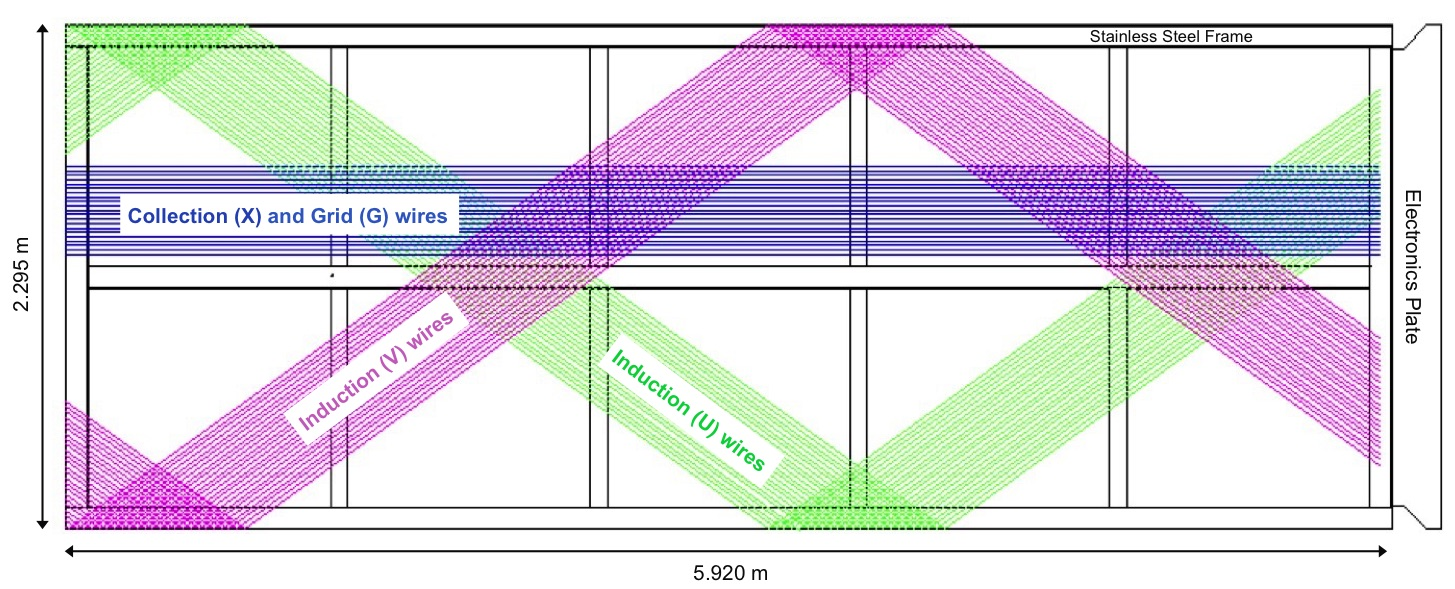
\includegraphics[width=0.95\textwidth]{APA-drawing-wire-configuration.jpg} 
%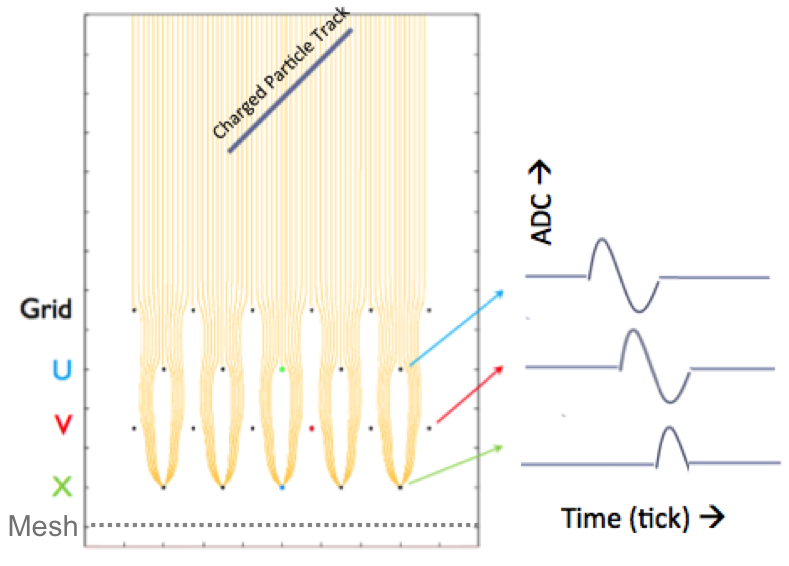
\includegraphics[height=0.185\textheight]{APA-drawing-wire-field-signals.png} 
%\includegraphics[width=0.8\textwidth, angle=90]{tpc_apa1} 
\end{dunefigure}

A complete list of APA design requirements can be found in DUNE-docdb-6416. Here we summarize the key design parameters and the considerations driving the main design choices for the APAs.  

\begin{itemize}
\item \textbf{APA size.} The size of the APAs is chosen for fabrication purposes, compatibility with over-the-road shipping, for eventual transport to the 4850 level at SURF and installation into the membrane cryostat of a detector module. %Sufficient shock absorption and clearances are taken into account at each stage.  
The dimensions are also chosen such that an integral number of electronic readout channels and boards fill in the full area of the APA. %The modularity of the APAs allows them to be built and tested at off-site production facilities, decoupling their manufacturing time from the construction of the membrane cryostat.

\item \textbf{Detector active area.} Coverage of the sensitive surface of the detector is achieved by tiling the area with multiple APAs. Dead regions due to frames, wire boards, electronics, and cabling are minimized, and APAs should be sensitive over most of the full area of an APA frame. The wrapped style allows all channels to be read out at the top of the APA, minimizing the amount of dead space between the APAs that would otherwise be occupied by electronics and associated cabling.    

%\item \textbf{System signal-to-noise.} The minimum required S/N for DUNE-SP is 9:1 to allow MIP measurement with high efficiency everywhere in the TPC. This sets a lower limit on the wire pitch, an upper limit on wire length, and requires use of a wire with low resistivity. 

\item \textbf{Wire angles.} The X wires run vertical to provide optimal reconstruction of beam-induced particle tracks, which are predominantly forward (in beam direction). The angle of the induction planes in the APA, $\pm35.7^{\circ}$, ensures that each induction wire only crosses a given collection wire once, reducing the ambiguities that the reconstruction must address.  The design angle of the induction wires, coupled with their pitch, was also chosen such that an integer multiple of electronics boards reads out one APA.
%The U,V wire angle of $\pm$35.7$^\circ$ is based on reducing reconstruction ambiguities and is chosen such that no induction wire crosses any collection wire more than once. Triplets of U,V,X wires never intersect more than once.

\item \textbf{Wire pitch.} The choice of wire pitch, approximately \SI{5}{mm}, combined with key parameters for other TPC systems (described in their respective sections of the TDR), can achieve the required signal-to-noise while providing good tracking resolution and good granularity for particle identification (particularly $e-\gamma$ separation). The DUNE-SP requirement that it be possible to determine the fiducial volume (via analysis) to $< 1\%$ implies a vertex resolution of $\approx 1.5$~cm along each coordinate direction. The $\leq 5$~mm wire pitch achieves this for the $y$ and $z$ coordinates.  The resolution on the drift-coordinate $x$ of a vertex or hit will be better than in the $y-z$ plane, due to the combination of drift-velocity and electronics sampling-rate.  Finally, the total number of wires on an APA must match the granularity of the electronics boards (each front-end motherboard can read out 128 wires, mixed between the $X,U,V$ planes). This determines the exact wire spacings of \SI{4.790}{mm} and \SI{4.669}{mm} on the collection and induction planes, respectively.  To achieve the reconstruction precision required (e.g. for $dE/dx$ reconstruction accuracy and multiple Coulomb scattering determination), the tolerance on the wire pitch is $\pm$\SI{0.5}{mm}.

In 2017, the DUNE Far Detector Task Force, utilizing a full Far Detector simulation and reconstruction chain, performed many detector optimization studies to quantify the impact of wire pitch and wire angle on physics performance.  The Task Force's final report is available in DUNE-docdb-3384, but their results indicate that a reduction in wire spacing (to \SI{3}{mm}) or change in wire angle (to 45$^\circ$) would not significantly impact the performance for the main physics goals of DUNE, including CP sensitivity.  Figure~\ref{fig:e-gamma}(b) reproduces their results showing the impact of wire pitch/orientations on electron-photon identification. The electron signal selection efficiency is shown as a function of the background rejection for different configurations. At a signal efficiency of $90\%$, the background rejection can be improved by $\approx 1\%$ using \SI{3}{mm} spacing or $45^\circ$ wire angles.  The conclusion that a slight improvement is possible with more dense hit information or more optimal wire angles is not surprising, but the impact on high-level physics sensitivities from this improvement are small. The conclusions of the Far Detector Task Force do not seem to justify the substantial cost impacts of making such changes to the DUNE detector design.        

\begin{dunefigure}[electron-gamma ID dependence on wire pitch and angle]{fig:e-gamma}{Summary of electron-$\gamma$ separation performance studies from the DUNE Far Detector Task Force (figures from DUNE-docdb-3384). (a): $e-\gamma$ separation by $dE/dx$ for the nominal wire spacing and angle (\SI{5}{mm}/$37.5^\circ$) compared to \SI{3}{mm} spacing or $45^\circ$ induction wire angles. (b) Electron signal selection efficiency versus photon (background) rejection for the different detector configurations.}
(a)
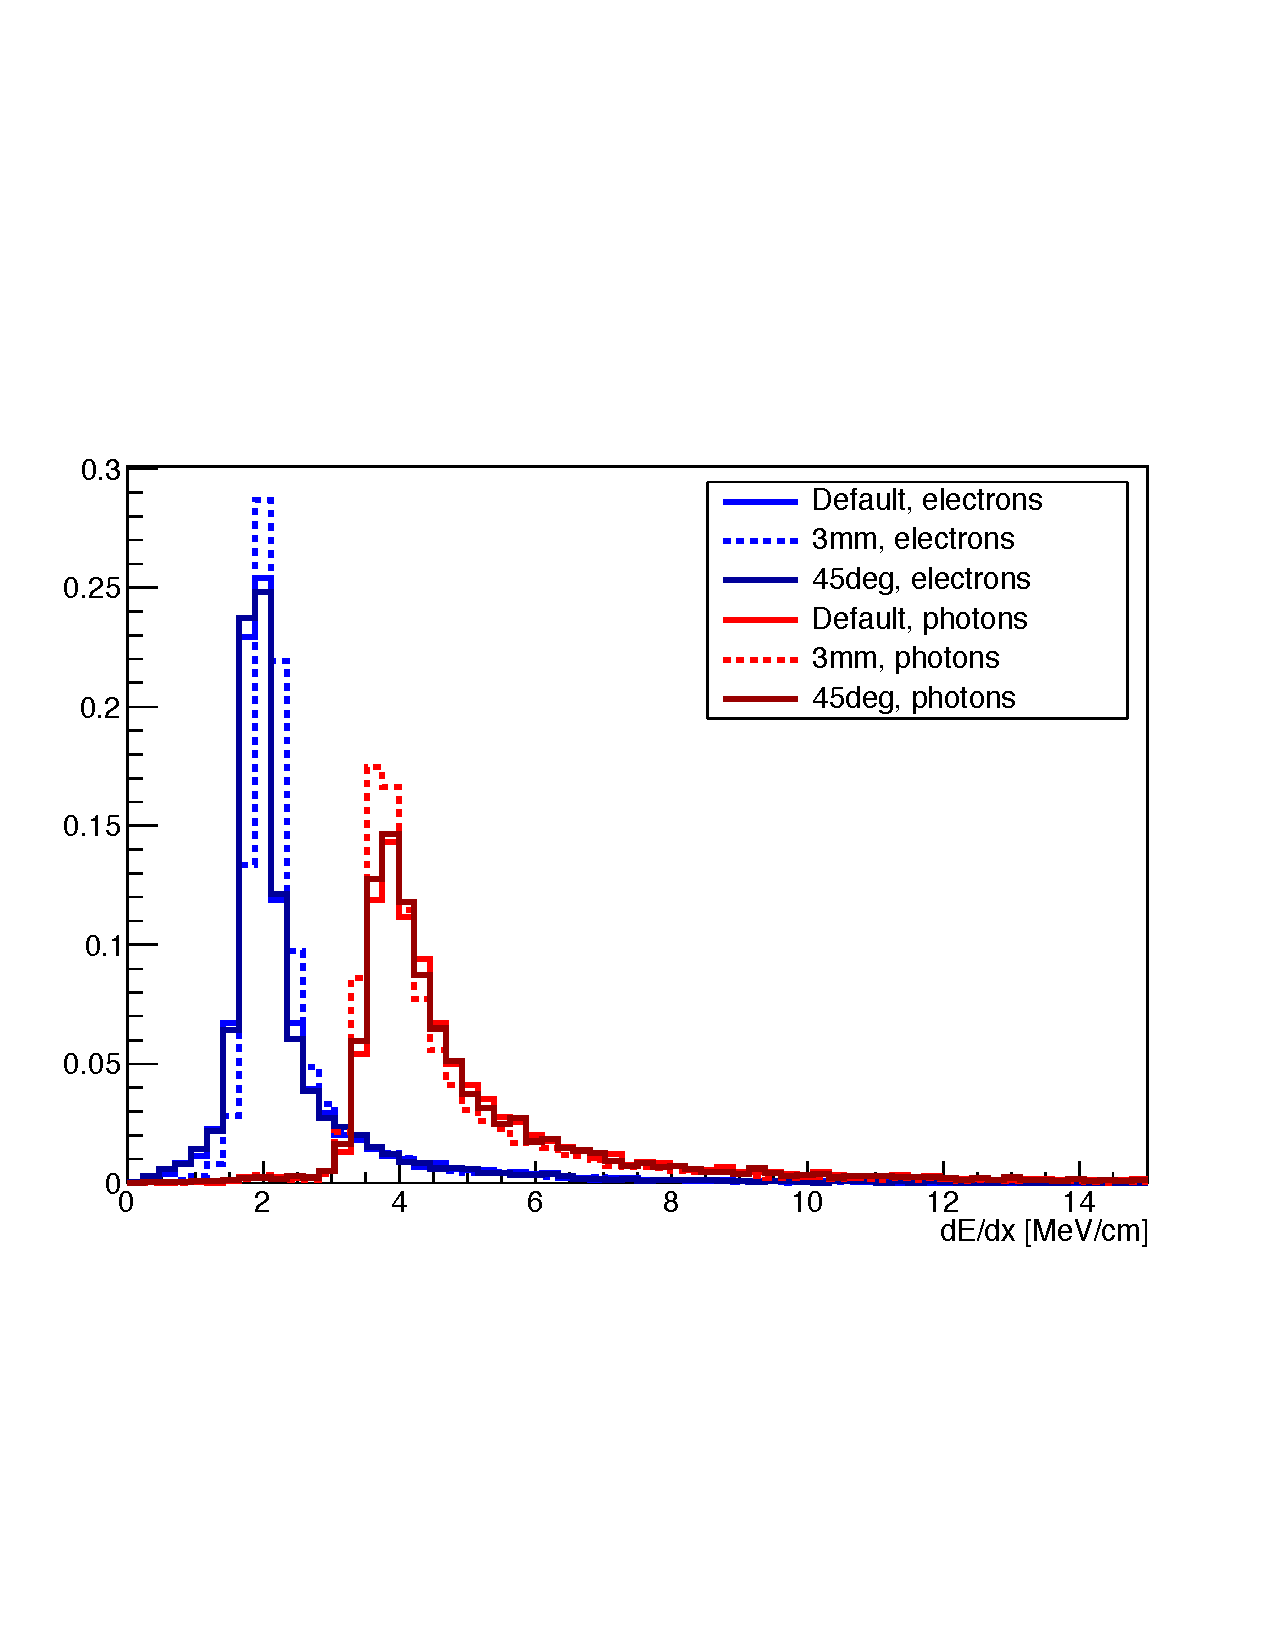
\includegraphics[height=0.23\textheight]{dEdx.pdf} \qquad
(b)
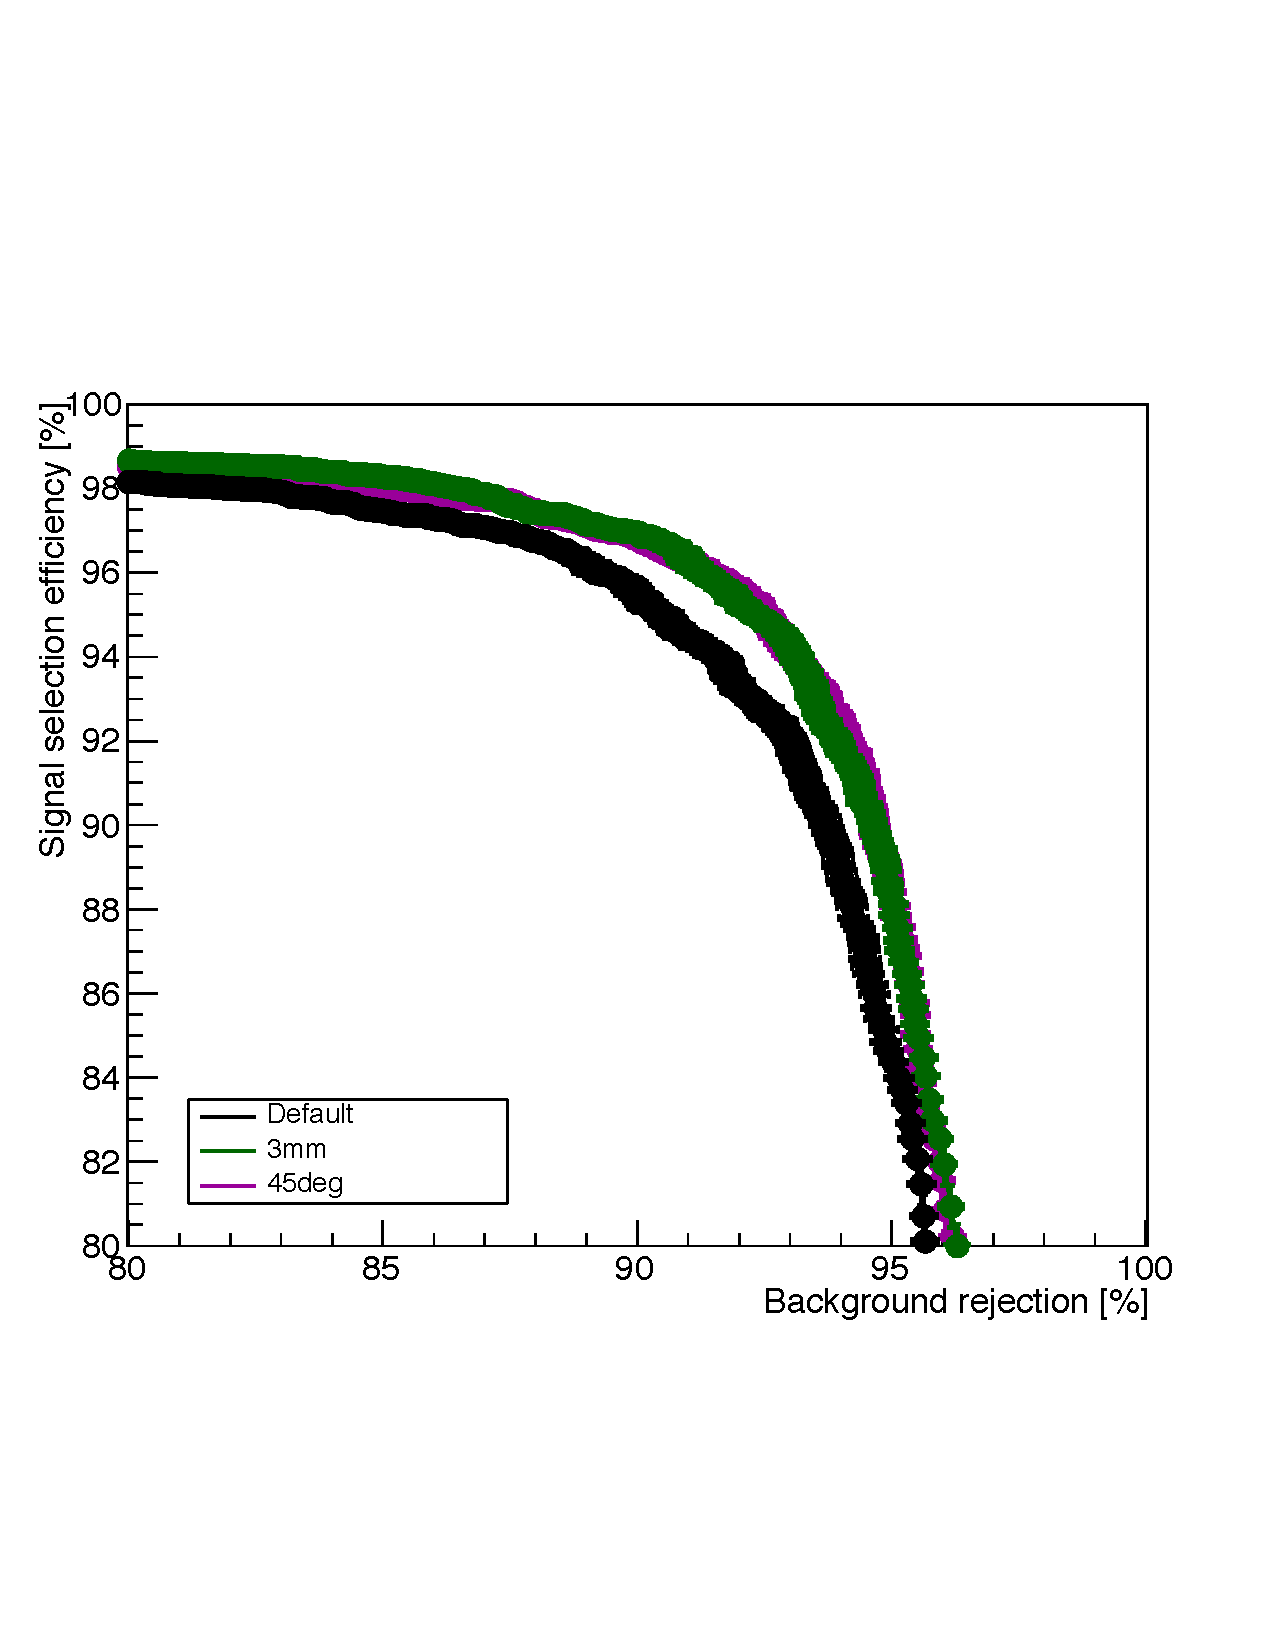
\includegraphics[height=0.23\textheight]{eff-bkgd-wires.pdf} 
\end{dunefigure}

\item \textbf{Wire plane transparency and signal shapes.}  The ordering of the layers, from the outside in, is $G-U-V-X$, followed by the mesh. The operating voltages of the APA layers are listed in Table~\ref{tab:bias}.  When operated at these voltages, the drifting ionization follows trajectories around the grid and induction wires, ultimately terminating on a collection plane wire. The grid and induction layers are completely transparent to drifting ionization, and the collection plane is completely opaque.  The grid layer is present for pulse-shaping purposes and not connected to the electronics readout. It effectively shields the first induction plane from the drifting charge and removing the long leading edge from the signals on that layer. The mesh layer shields the sense planes from pickup from the photon detection system and from ``ghost'' tracks that would otherwise be visible when ionizing particles have a trajectory that passes through the collection plane. Figure~\ref{fig:apa-fields} shows the field simulation and expected signal shapes for the bias voltages listed in Table~\ref{tab:bias}.

\begin{table}[ht]
\begin{minipage}[b]{0.46\linewidth}
\centering
\begin{tabular}{ l  r }
    \hline
    \textbf{Anode Plane} & \textbf{Bias Voltage (V)} \\ \toprowrule
	Grid ($G$) & -665 \\ \colhline
	Induction ($U$) & -370 \\ \colhline
	Induction ($V$) & 0 \\ \colhline
	Collection ($X$) & 820 \\ \colhline
	Mesh ($M$) & 0 V\\ \colhline
    \end{tabular}
    \caption{Baseline bias voltages for APA wire layers.}
    \label{tab:bias}
\end{minipage}\hfill
\begin{minipage}[t]{0.5\linewidth}
\centering
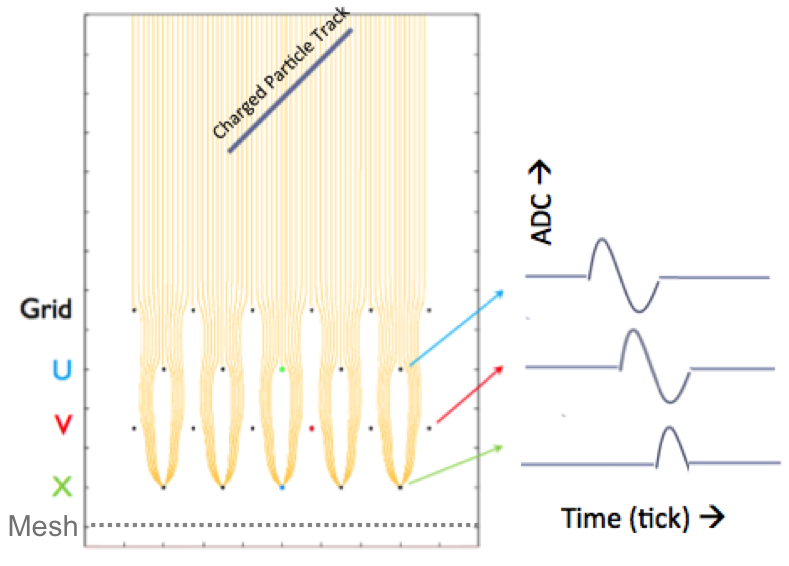
\includegraphics[width=0.9\linewidth]{APA-drawing-wire-field-signals.png}
\captionof{figure}{Field lines and signal shapes on the APA induction and collection wires.}
\label{fig:apa-fields}
\end{minipage}
\end{table}

\begin{comment}
\begin{dunetable}[Baseline bias voltages for APA wire layers]{lr}{tab:bias}{Baseline bias voltages for APA wire layers.}   
Anode Plane & Bias Voltage  \\ \toprowrule
Grid (G) & -665 V\\ \colhline
Induction (U) & -370 V\\ \colhline
Induction (V) & 0 V\\ \colhline
Collection (X) & 820 V\\ \colhline
Mesh (M) & 0 V\\
\end{dunetable}

\begin{dunefigure}[Wire plane field lines and signal shapes]{fig:apa-fields}{Field lines and signal shapes on the APA induction and collection wires.}
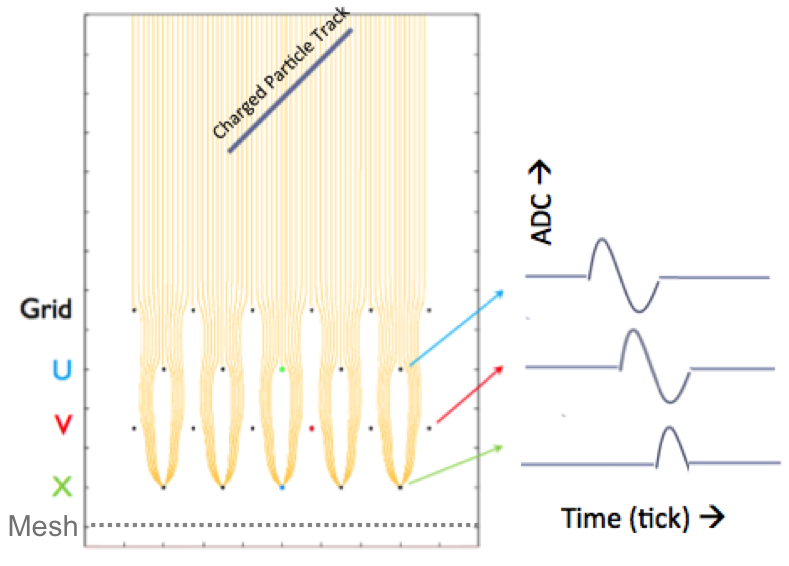
\includegraphics[width=0.5\textwidth]{APA-drawing-wire-field-signals.png} 
\end{dunefigure}
\end{comment}

\item \textbf{Wire type.}  The sense wires on the APA are \SI{150}{$\mu$m} beryllium (1.9\%) copper wire, %\footnote{\url{http://www.lfa-wire.com/heat-treatable-alloy-25_c17200-and-c17300.htm}}
chosen for its mechanical and electrical properties, the ability to solder, and cost.  See Section~\ref{sec:fdsp-apa-wires} for more information.

\item \textbf{Wire tension.} The nominal wire tension of \SI{5}{N}, when combined with the intermediate support combs (described in Section~\ref{sec:combs}) ensure that the wires are held taught in place with no sag.  Wire sag can impact the precision of reconstruction, as well as the transparency of the TPC.  The tension of \SI{5}{N} is low enough that when the wires are cooled, which increases their tension due to thermal contraction, they will stay safely below the break load of the beryllium copper wire.  To further mitigate wire breakage and its impact on detector performance, each wire in the APA is anchored twice on both ends, with both solder and epoxy.

\end{itemize}


The principal design parameters for the DUNE APAs are summarized in Table~\ref{tab:apaparameters}.

\begin{dunetable}[APA design parameters]{lr}{tab:apaparameters}{APA design parameters}   
Parameter & Value  \\ \toprowrule
Active Height & 5.984 m\\ \colhline
Active Width & 2.300 m\\ \colhline
Wire Pitch (U,V) & 4.669 mm\\ \colhline
Wire Pitch (X,G) & 4.790 mm\\ \colhline
Wire Position Tolerance & 0.5 mm \\ \colhline
Wire Plane Spacing & 4.75 mm\\ \colhline
Wire Angle (w.r.t. vertical) (U,V) & 35.7$^{\circ}$\\ \colhline
Wire Angle (w.r.t. vertical) (X,G) & 0$^{\circ}$\\ \colhline
Number Wires / APA & 960 (X), 960 (G), 800 (U), 800 (V) \\ \colhline
Number Electronic Channels / APA & 2560 \\ \colhline
Wire Tension & 5.0 N \\ \colhline
Wire Material & Beryllium Copper \\ \colhline
Wire Diameter & 150 $\mu$m \\ \colhline
Wire Resistivity & 7.68 $\mu\Omega$-cm $@$ 20$^{\circ}$ C \\ \colhline
Wire Resistance/m & 4.4 $\Omega$/m $@$ 20$^{\circ}$ C \\ \colhline
Frame Planarity & 5 mm \\ \colhline
Photon Detector Slots & 10 \\
\end{dunetable}


%An APA is constructed from a framework of lightweight, rectangular stainless steel tubing, with a fine mesh covering the rectangular area within the frame, on both sides, that defines a uniform ground across the frame. Along the length of the frame and around it, over the mesh layer, layers of sense and shielding wires are strung or wrapped at varying angles relative to each other, as illustrated in  Figure~\ref{fig:tpc_apa1}. The wires are terminated on  boards that anchor them and also provide the connections to the readout electronics. The APAs are approximately \SI{2.3}{m} wide, \SI{6.0}{m} high, and \SI{12}{cm} thick.  

%Starting from the outermost wire layer, there is first a shielding (grid) plane, followed by two induction planes, and finally the collection plane. All wire layers span the entire height of the APA frame. The layout of the wire layers is illustrated in  Figure~\ref{fig:tpc_apa1}.

%The angle of the induction planes in the APA ($\pm$35.7$^{\circ}$) is chosen such that each induction wire only crosses a given collection wire one time, reducing the ambiguities that the reconstruction must address.  The design angle of the induction wires, coupled with their pitch, was also chosen such that an integer multiple of electronics boards reads out one APA.

%The wires of the grid (shielding) layer, G,  are not connected to the electronic readout; the wires run parallel to the long edge of the APA frame; there are separate sets of G wires on the two sides of the APA. 
%The two planes of induction wires (U and V) wrap in a helical fashion around the long edge of the APA, continuously around both sides of the APA.  The collection plane wires (X) run vertically, parallel to G.   The ordering of the layers, from the outside in, is G-U-V-X, followed by the mesh.   

%The operating voltages of the APA layers are listed in Table~\ref{tab:bias}.  When operated at these voltages, the drifting ionization follows trajectories around the grid and induction wires, ultimately terminating on a collection plane wire; i.e., the grid and induction layers are completely transparent to drifting ionization, and the collection plane is completely opaque.  The grid layer is present for pulse-shaping purposes, effectively shielding the first induction plane from the drifting charge and removing the long leading edge from the signals on that layer; again, it is not connected to the electronics readout. The mesh layer serves to shield the sense planes from pickup from the Photon Detection System and from ``ghost'' tracks that would otherwise be visible when ionizing particles have a trajectory that passes through the collection plane. 

\begin{comment}
\begin{dunetable}[Baseline bias voltages for APA wire layers]{lr}{tab:bias}{Baseline bias voltages for APA wire layers}   
Anode Plane & Bias Voltage  \\ \toprowrule
Grid (G) & -665 V\\ \colhline
Induction (U) & -370 V\\ \colhline
Induction (V) & 0 V\\ \colhline
Collection (X) & 820 V\\ \colhline
Mesh (M) & 0 V\\
\end{dunetable}

\begin{dunefigure}[APA diagram]{fig:apa-fields}
{Field lines and signal shapes on the APA induction and collection wires.}
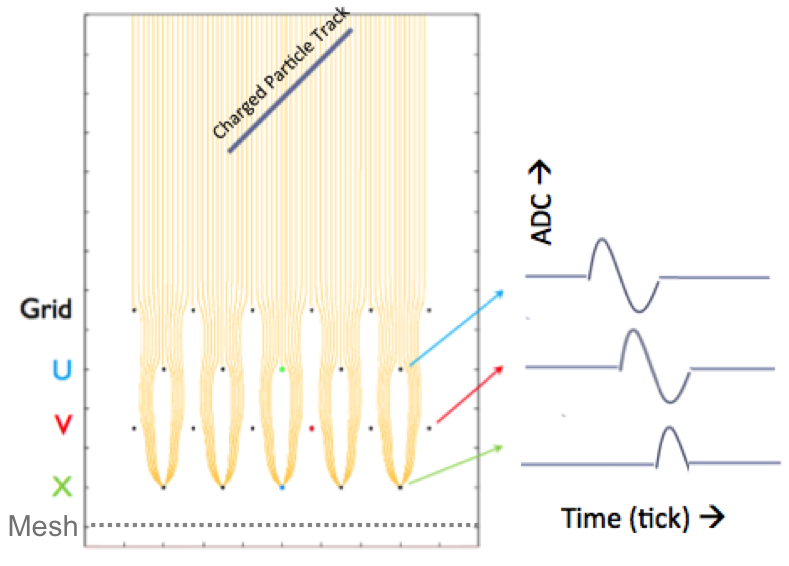
\includegraphics[width=0.5\textwidth]{APA-drawing-wire-field-signals.png} 
\end{dunefigure}
\end{comment}

%The wrapped style allows the APA plane to fully cover the active area of the LArTPC, minimizing the amount of dead space between the APAs that would otherwise be occupied by electronics and associated cabling.   

%In the current design of the DUNE-SP far detector module, a central row of APAs is flanked by  drift-fields, requiring sensitivity on both sides. The wrapped APAs allow the induction plane wires to sense drifting ionization originating from either side of the APA.  This double-sided feature is not strictly necessary for the APAs located against the cryostat walls with a drift field on one side only, but it is compatible with this setup as the grid layer facing the wall effectively blocks any ionization generated outside the TPC from drifting in to the wires on that side of the APA.

%The choices of wire tension and wire placement accuracy are made to ensure proper operation of the LArTPC at voltage, and to provide the precision necessary for reconstruction.  The tension of 5\,N, when combined with the intermediate support combs (described in Section~\ref{subsec:apa_combs}) ensure that the wires are held taught in place with no sag.  Wire sag can impact the precision of reconstruction, as well as the transparency of the TPC.  The tension of 5~N is low enough that when the wires are cooled, which increases their tension due to thermal contraction, they will stay safely below the break load of the beryllium copper wire, as described in Section~\ref{subsec:apa_wires}.  To further mitigate wire breakage and its impact on detector performance, each wire in the APA is anchored twice on both ends, with both solder and epoxy.  


%%%%%%%%%%%%%%%%%%%%%%%%%%%%%%%%%%%
\subsection{APA Frames}
\label{sec:fdsp-apa-frames}

The APA frames are a bolted assembly of rectangular hollow section (RHS) stainless steel tubes.  As seen in Figures~\ref{fig:apa-frame} and \ref{fig:apa-frame-2}, there are three long tubes, a foot tube, a head tube, and eight cross-pieces that create the \SI{6.06}{m} tall by \SI{2.30}{m} wide frame. 

\begin{dunefigure}[APA dimensions]{fig:apa-frame}{A drawing of an APA frame showing the main components. }
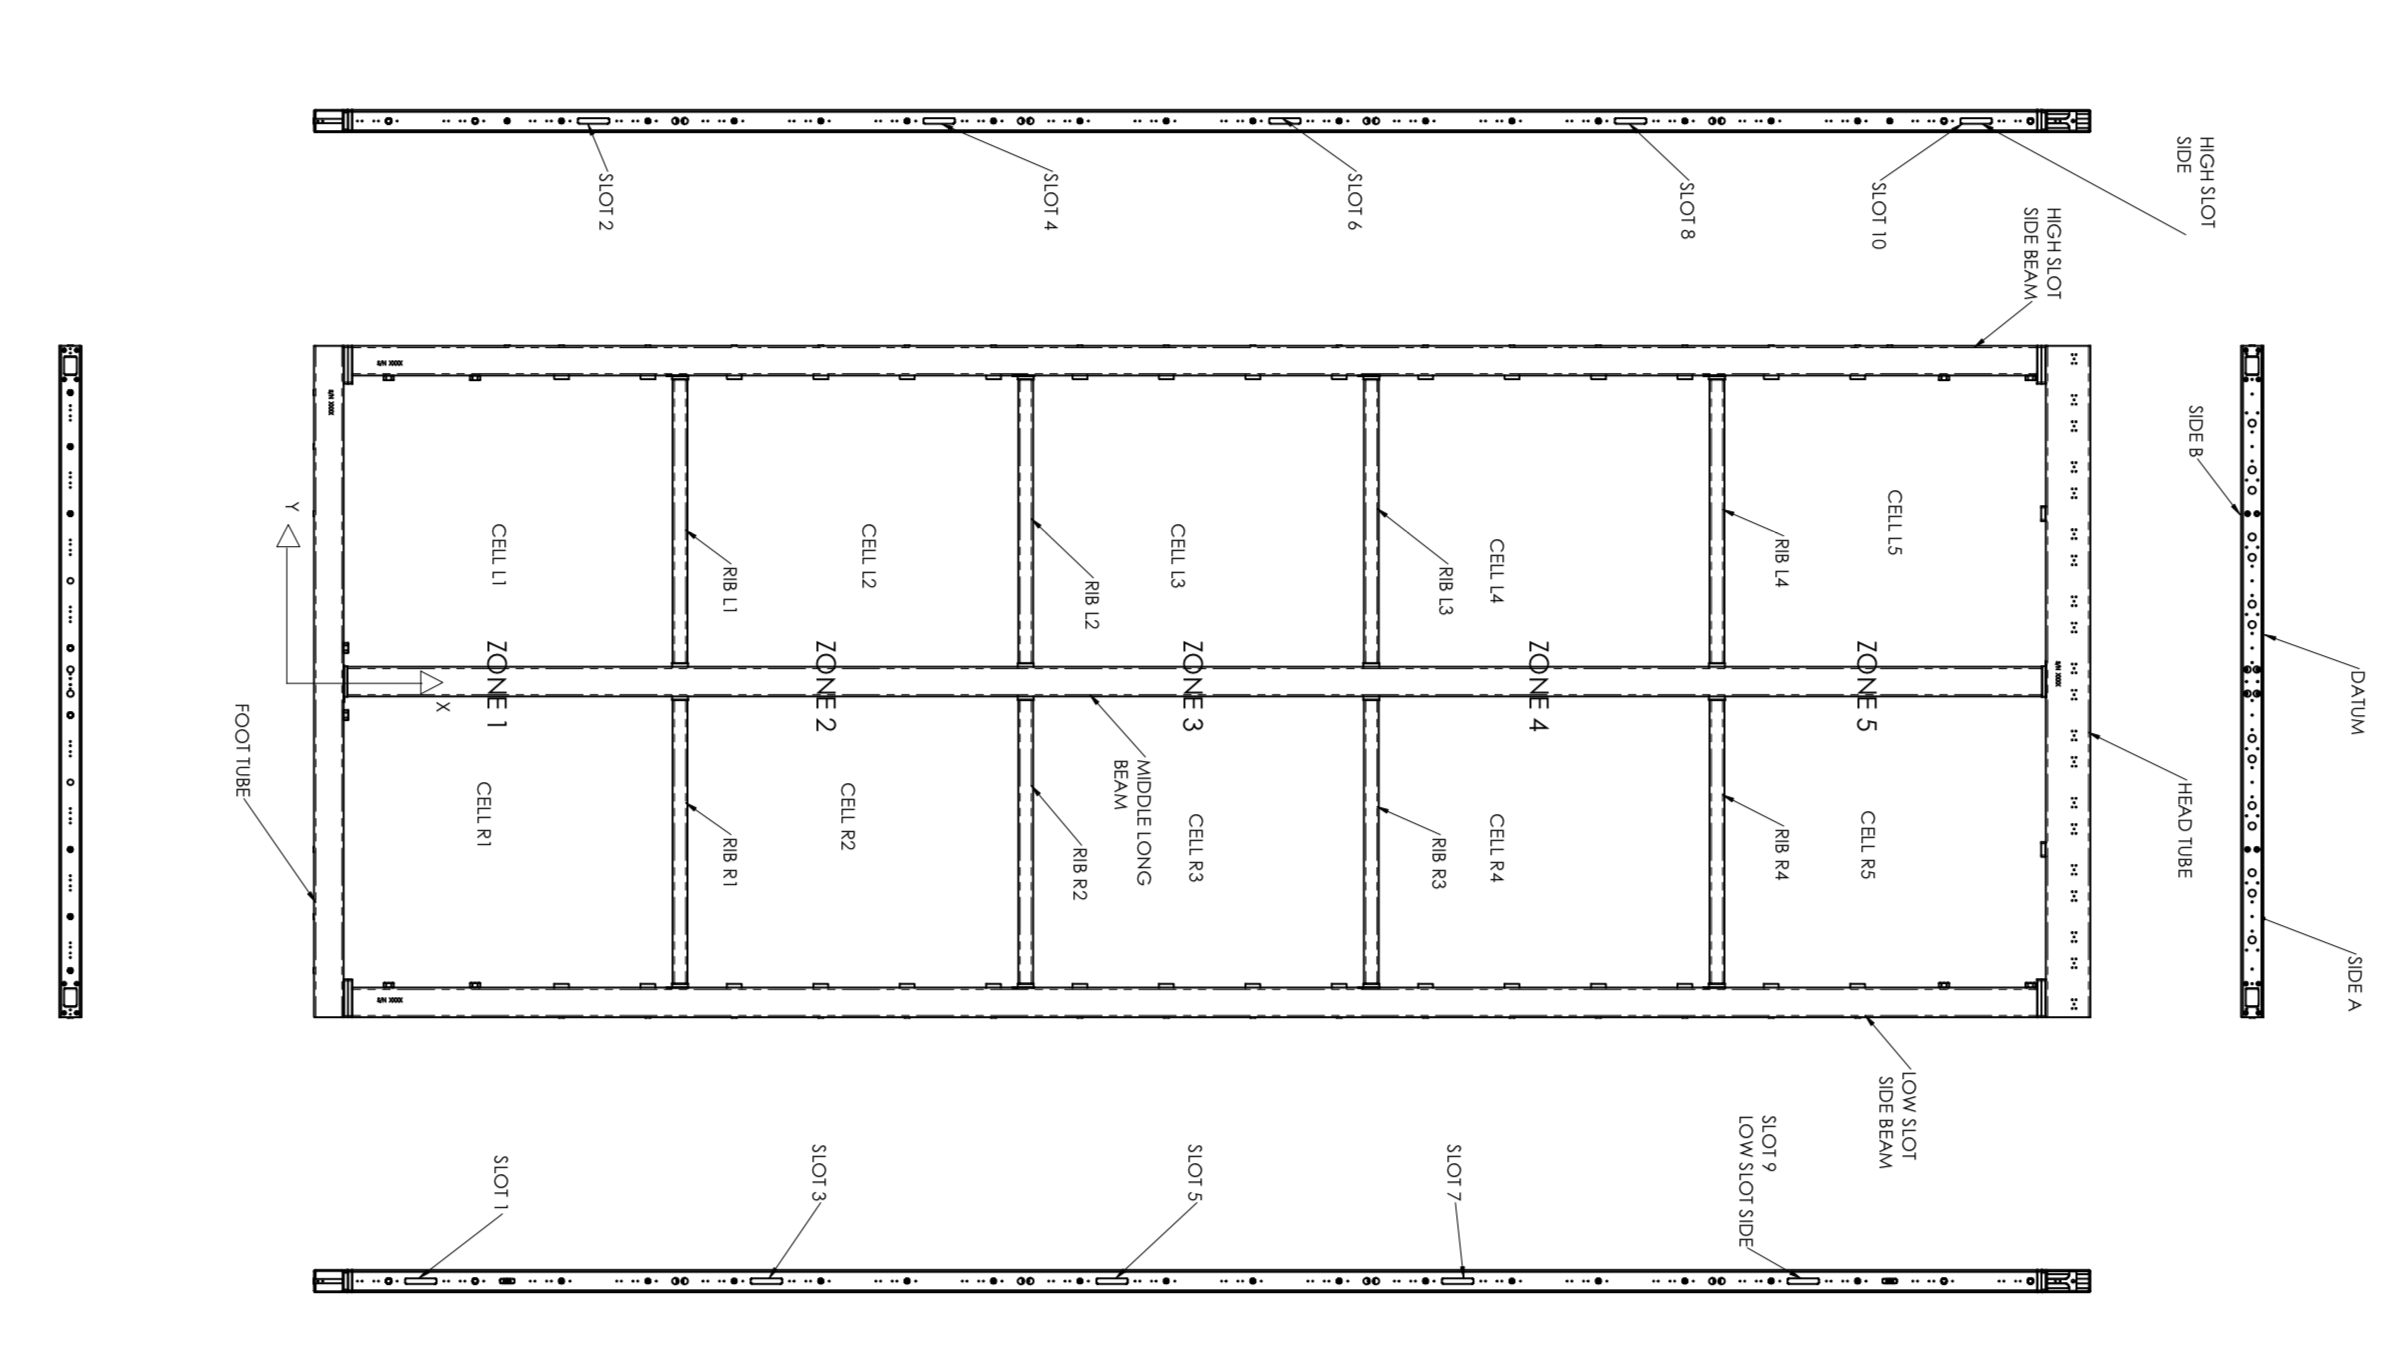
\includegraphics[width=1.3\textwidth, angle=90]{APAFrameDimensions} 
\end{dunefigure}

The dimensions of the RHS to be used are currently being revisited from that used in ProtoDUNE due to the additional requirements on the frames in the DUNE far detector.  The baseline design of 3 x 4 in. RHS with 0.120 in. wall-thickness tubing, as used for the outer tubes in ProtoDUNE, will create challenges for cable routing in the double-height APA assembly required in DUNE.  The current options under consideration are increasing the profile of the outer tubes to 3 x 5 in., which does not impact the fiducuial volume of the detector, or to 4 x 4 in., which will decrease the fiducial volume by 0.5\%.  The four central cross-pieces are made from 2 x 3 in. RHS, and are likely to be unaffected by the scaleup. The robustness of the amended frame in both options is currently undergoing engineering analysis.  

\begin{dunefigure}[APA frame]{fig:apa-frame-2}{An APA frame showing overall dimensions.}
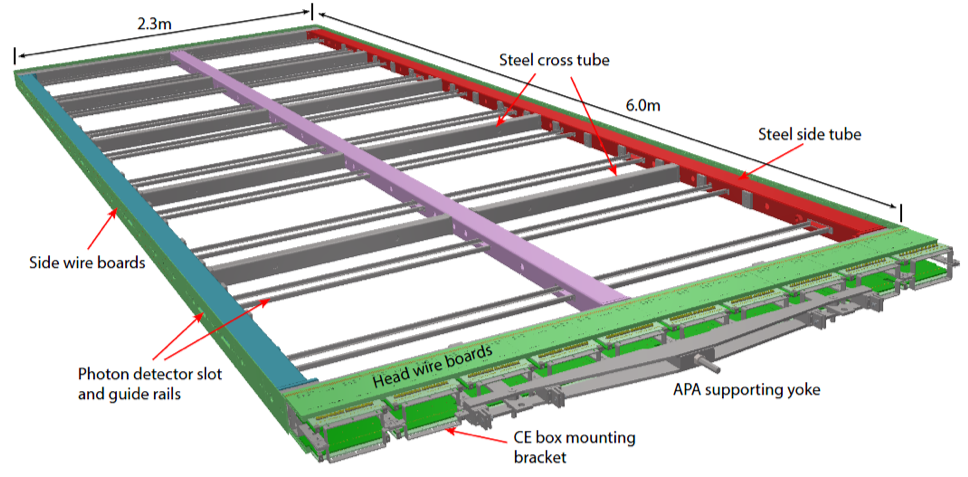
\includegraphics[width=\textwidth]{APAFrameDrawing} 
\end{dunefigure}

The head and foot tubes are attached to the side and center tubes via welded abutment flanges, which are shimmed to create a flat, rectangular frame of the specified dimensions (Figure~\ref{fig:tpc_apa_boltedjointdrawing}, left).  The central cross-pieces are attached to the side pieces in a similar manner (Figure~\ref{fig:tcp_apa_boltedjointdrawing}, right).  In production, the pieces are individually machined, and cleaned prior to assembly, which gives flexibility both in the production processes and in terms of achieving the flatness necessary.  

\begin{dunefigure}[APA bolted joint drawings]{fig:tpc_apa_boltedjointdrawing}{Models of the bolted joints. The holes on the top of the tube are for access to tighten the screws. The heads actually tighten against the lower hole, inside the tube.}
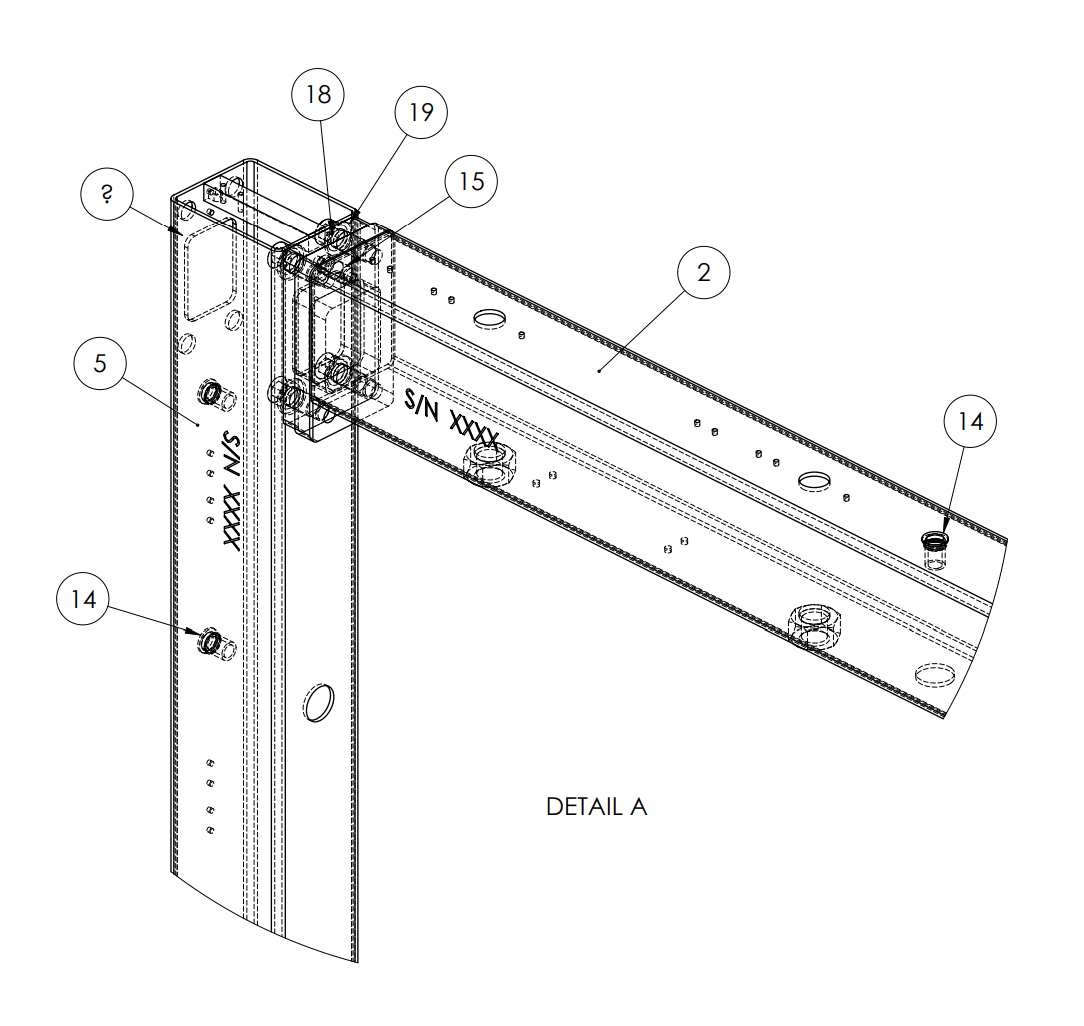
\includegraphics[width=0.45\textwidth]{BoltedJointCorner} 
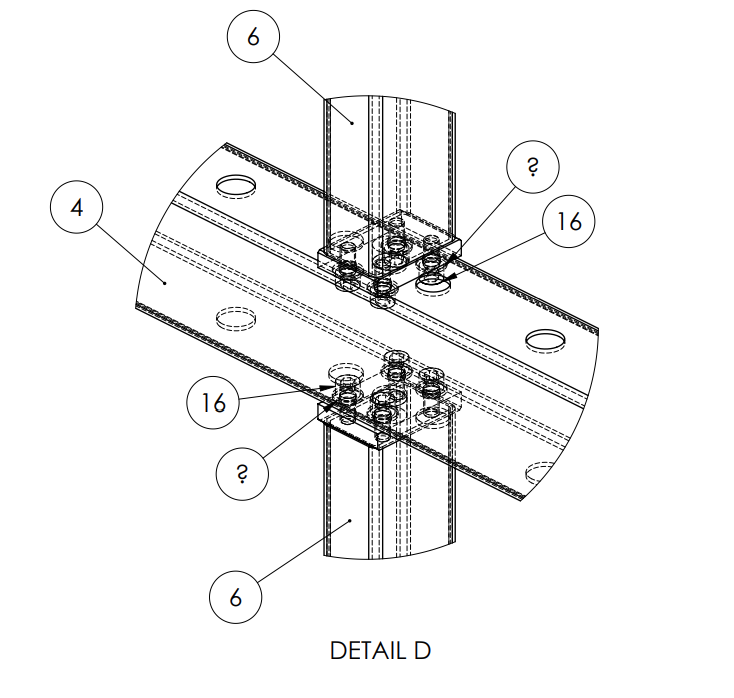
\includegraphics[width=0.45\textwidth]{BoltedJointSide} 
\end{dunefigure}

The APA frames are used both as the support structure for the wire plane readout and photon detector system, as well as for routing cables for both of these systems. The foot tubes of two APA frames will be mechanically connected to form a 12~m tall structure, as shown in Figure~\ref{fig:tpc_apa_dual}, and these assemblies are mounted edge to edge to form a continuous plane. 

\begin{dunefigure}[Dual APA diagram]{fig:tpc_apa_dual}{Diagram of an APA pair, with bottom APA hung from the top APA. The dimensions of the APA pair and accompanying electronics and mechanical supports are indicated.}
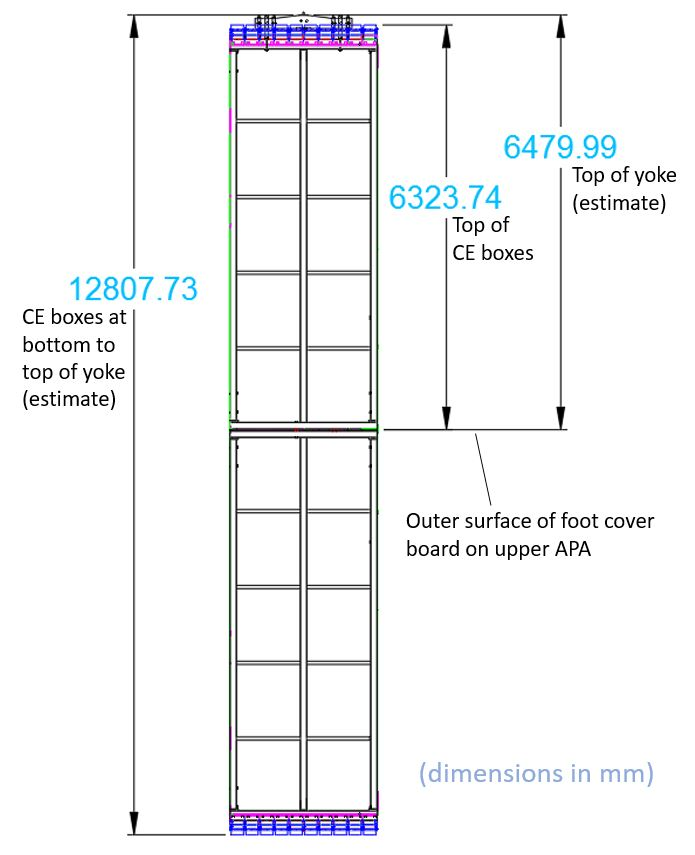
\includegraphics[width=0.9\textwidth]{Dual_APA_dimensioned.jpg} 
\end{dunefigure}


%%%%%%%%%%%%%%%%%%%%%%%%%%%%%%%%%%%%%%%
\subsection{Grounding mesh}
\label{sec:fdsp-apa-mesh}

A fine mesh screen is glued directly to the steel frame surface, over the frame on both sides.  It creates a uniform ground layer beneath the wire planes, and also mitigates against 'ghost' tracks as charged particles ionise the argon between the inner wire layers.

The mesh is installed in four parts, along the length of the left- and right-hand halves of each side of the APA. The mesh is clamped around the perimeter of the opening and then pulled tight (by opening and closing clamps as needed during the process).  When the mesh is taut, a \SI{25}{mm}-wide strip is masked off around the opening and epoxy is applied through the mesh to attach it to the steel.  Although measurements have shown that this gives good electrical contact between the mesh and the frame, a deliberate electrical connection is also made.  Figure~\ref{fig:tpc-apa-mesh-application} depicts the mesh application setup for a full-size ProtoDUNE-SP APA.

\begin{dunefigure}[APA mesh application]{fig:tpc-apa-mesh-application}{Left: mesh being clamped to the APA. Right: mesh being taped off, ready for gluing.}
\setlength{\fboxsep}{0pt}
\setlength{\fboxrule}{0.5pt}
\fbox{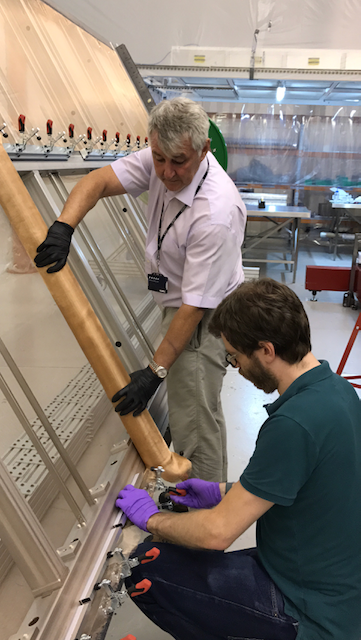
\includegraphics[height=0.6\textwidth]{MeshApplication}} 
\fbox{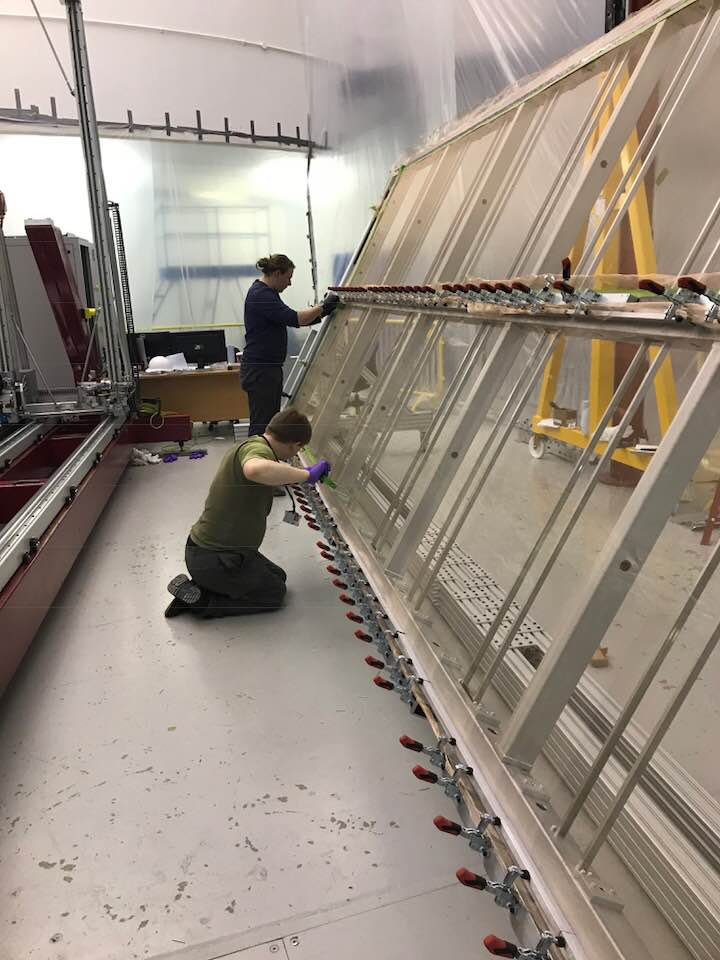
\includegraphics[height=0.6\textwidth]{MeshApplied}}
\end{dunefigure}

The mesh installation procedure described above is difficult, and prone to bumps being left in the mesh that can short against the x-layer. For the DUNE mass production, a window-frame design is being considered, where mesh is pre-stretched over smaller sub-frames that can be clipped into each gap between cross-beams in the full APA frame.


%%%%%%%%%%%%%%%%%%%%%%%%%%%%%%%%%%%
\subsection{Wires}
\label{sec:fdsp-apa-wires}

Beryllium copper (CuBe) wire is known for its high durability and yield strength. It is composed of $\sim$98$\%$ copper, 1.9$\%$ beryllium, and a negligible amount of other elements. The APA wire has a diameter of \SI{150}{$\mu$m} (\SI{.006}{in.}), and is strung in varying lengths across the APA frame. Three key properties for its usage in the APA are: low resistivity, high tensile or yield strength, and coefficient of thermal expansion suitable for use with the APA's stainless steel frame.

Tensile strength of the wire describes the wire-breaking stress (see Table~\ref{tab:wire}).  The yield strength is the stress at which the wire starts to take a permanent (inelastic) deformation, and is the important limit stress for this case, though most specifications give tensile strength.  Fortunately, for the CuBe alloys of interest, the two are fairly close to each other.  Based on the tensile strength of wire purchased from Little Falls Alloy (over \SI{1,380}{MPa} or \SI{200,000}{psi}), the yield strength is greater than \SI{1,100}{MPa}.  Given that the stress while in use is around \SI{280}{MPa}, this leaves a comfortable margin.

The coefficient of thermal expansion (CTE) describes how material expands and contracts with changes in temperature.  The CTEs of CuBe alloy and 304 stainless steel are very similar.  Integrated down to \SI{87}{K}, they are \SI{2.7}{mm/m} for stainless and \SI{2.9}{mm/m} for CuBe~\cite{cryo-mat-db}. Since the wire contracts slightly more than the frame, during cool-down the wire tension increases.  For wires starting at \SI{5}{N} at room temperature, the tension increases to around \SI{5.5}{N} when everything reaches LAr temperature.  

The change in wire tension during cool-down could also be a concern.  In the worst case, the wire cools quickly to \SI{87}{K} before any significant cooling of the frame  -- a realistic case because of the differing thicknesses.  In the limiting case, with complete contraction of the wire and none in the frame, the tension would be expected to peak at $\sim$\SI{11.7}{N}, which is still well under the $\sim$\SI{20}{N} yield tension. In practice, the cooling will be done gradually to avoid this tension spike as well as other thermal shock to the APA.

\begin{dunetable}[CuBe wire tensile strength and CTE]{lr}{tab:wire}{Tensile strength and coefficient of thermal expansion (CTE) of beryllium copper (CuBe) wire.}
Parameter & Value \\ \toprowrule
Tensile Strength (from property sheets) (psi) & 208,274 \\ \colhline
Tensile Strength (from actual wire) (psi) & 212,530 \\ \colhline
CTE of CuBe, integrated to 87 K (m/m) & 2.9e-3 \\ \colhline
CTE of 304 stainless steel, integrated to 87 K (m/m) & 2.7e-3 \\
\end{dunetable}



%%%%%%%%%%%%%%%%%%%%%%%%%%%%%%%%%%%
\subsection{Anchoring Elements and Wire Boards}
\label{sec:fdsp-apa-boards}

%\fixme{Include an image of the subsystem (boards), indicating its parts. Show how the system fits into the overall system (APA).}

%%%%%%%%%%%%
\subsubsection{Head Electronics Boards}

At the head end of the APA, stacks of electronics boards (referred to as ``wire boards'') are arrayed to anchor the wires.  They also provide the connection between the wires and the cold electronics.

All APA wires are terminated on the wire boards, which are stacked along the electronics end of the APA frame (see Figure~\ref{fig:tpc_apa_boardstack}). Attachment of the wire boards begins with the X plane (innermost). After the X-plane wires are strung top to bottom along each side of the APA frame, they are soldered and epoxied to their wire boards and trimmed. The remaining wire board layers are attached as each layer is wound.  The main CR boards (capacitive-resistive), which provide DC bias and AC coupling to the wires, are attached to the bottom of the wire board stack. 

\begin{dunefigure}[APA board stack]{fig:tpc_apa_boardstack}{The APA wire board stack at the head end.}
\setlength{\fboxsep}{0pt}
\setlength{\fboxrule}{0.5pt}
\fbox{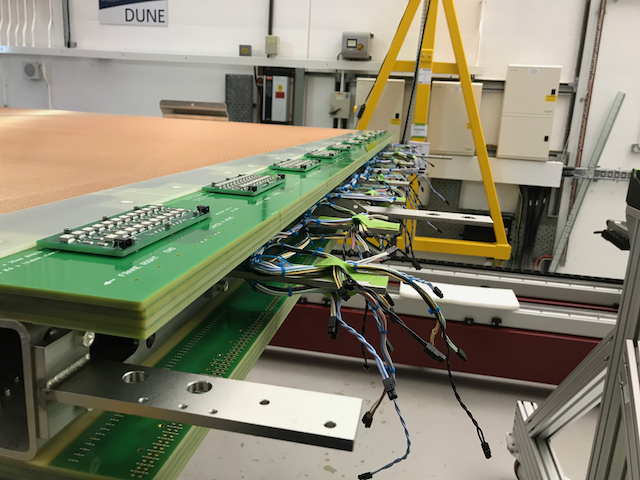
\includegraphics[width=0.7\textwidth]{APABoardStack}}
\end{dunefigure}

The outermost G-plane wire boards connect adjacent groups of four wires together, and bias each group through an R-C filter whose components are placed on special CR boards that are attached after the wire plane is strung. The X, U and V layers of wires are connected to the CE (housed in boxes mounted on the APA) either directly or through DC-blocking capacitors. The X and U planes have wires individually biased through \SI{50}{M$\Omega$} resistors. Electronic components for the X- and U-plane wires are located on a common CR board. 

Mill-Max pins and sockets provide electrical connections between circuit boards within a stack. They are pressed into the circuit boards and are not repairable if damaged. To minimize the possibility of damaged pins, the boards are designed so that the first wire board attached to the frame has only sockets. All boards attached subsequently contain pins that plug into previously mounted boards. This process eliminates exposure of any pins to possible damage during winding, soldering, or trimming processes.

Ten stacks of wire boards are installed across the width of each side along the head of the APA.  The X-layer board in each stack has room for 48 wires, the V layer has 40 wires, the U layer 40 wires and the G layer 48 wires.  Each board stack, therefore, has 176 wires but only 128 signal channels since the G wires are not read out. With a total of 20 stacks per APA, this results in \SI{2,560} signal channels per APA and a total of \SI{3,520} wires starting at the top of the APA and ending at the bottom.  There is a total of $\sim$\SI{23.4}{km} of wire on the two surfaces of each APA.  Many of the capacitors and resistors that in principle could be on these wire boards are instead placed on the attached CR boards to improve their accessibility in case of component failure.   Figure~\ref{fig:tpc_apa_electronics_connectiondiagram} depicts the connections between the different elements of the APA electrical circuit. 

\begin{dunefigure}[APA wire board connection to electronics]{fig:tpc_apa_electronics_connectiondiagram}{Diagram of the connection between the APA wires, viewed from the APA edge. The set of wire boards within a stack can be seen on both sides of the APA, with the CR board extending further to the right, providing a connection to the cold electronics, which are housed in the boxes at the far right of the figure. }
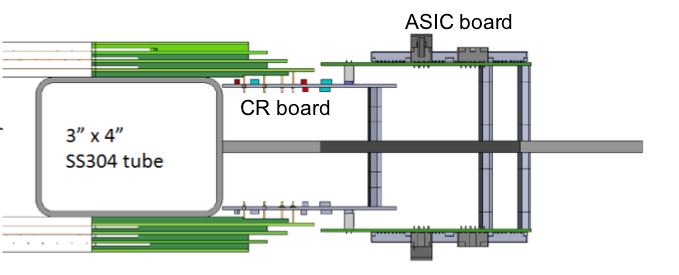
\includegraphics[width=0.8\textwidth]{BoardConnections}
\end{dunefigure} 

At the head end of the APA, the wire-plane spacing is set by the thickness of these wire boards.  The first layer's wires solder to the surface of the first board, the second layer's wires to the surface of the second board, and so on.  For installation, temporary toothed-edge boards beyond these wire boards align and hold the wires until they are soldered to pads on the wire boards.  After soldering, the extra wire is snipped off. 



%%%%%%%%%%%%%%%%
\subsubsection{CR Boards}
\label{sec:crboards}

The CR boards carry a bias resistor and a DC-blocking capacitor for each wire in the X and U planes. These boards are attached to the board stacks after fabrication of all wire planes.  Electrical connections to the board stack are made though Mill-Max pins that plug into the wire boards. Connections from the CR boards to the CE are made through a pair of 96-pin Samtec connectors.

Surface-mount bias resistors on the CR boards have resistance of \SI{50}{M$\Omega$} and are constructed with a thick film on a ceramic substrate. Rated for \SI{2.0}{kV} operation, the resistors measure 0.12 $\times$ \SI{0.24}{inches}. Other ratings include operation from $-$55 to +155 C, 5\% tolerance, and a \SI{100}{ppm/C} temperature coefficient. Performance of these resistors at LAr temperature is verified through additional bench testing.

The selected DC-blocking capacitors have capacitance of \SI{3.9}{nF} and are rated for \SI{2.0}{kV} operation. Measuring 0.22 $\times$ \SI{0.25}{inches} across and \SI{0.10}{inches} high, the capacitors feature flexible terminals to comply with PC board expansion and contraction. They are designed to withstand 1,000 thermal cycles between the extremes of the operating temperature range. Tolerance is also 5\%.

In addition to the bias and DC-blocking capacitors for all X- and U-plane wires, the CR board includes two R-C filters for the bias voltages. The resistors are of the same type used for wire biasing except with a resistance of \SI{2}{M$\Omega$}. Capacitors are \SI{47}{nF} at \SI{2}{kV}. Very few choices exist for surface-mount capacitors of this type, and they are exceptionally large. Polyester or Polypropylene film capacitors that are known to perform well at cryogenic temperatures are used.


%%%%%%%%%%%%%%%%%%%%%%%%
\subsubsection{Side and Foot Boards}

The boards along the sides and foot of the APA have notches, pins, and other location features to hold the wires in the correct position as they wrap around the edge from one side of the APA to the other.  G10 circuit board material is ideal for these side and foot boards due to its physical properties. 

A number of hole or slot features are needed in the edge boards to provide access to the underlying frame.  In order that these openings are not covered by wires, the sections of wire that would go over the openings are replaced by traces on the boards.  After the wires are wrapped, the wires over the opening are soldered to pads at the ends of the traces, and the section of wire between the pads is snipped out (see Figure~\ref{fig:tpc_apa_sideboardmodel}).  These traces are easily and economically added to the boards by the many commercial fabricators who make circuit boards. 

\begin{dunefigure}[APA side boards with traces that connect wires around openings]{fig:tpc_apa_sideboardmodel}{Side boards with traces that connect wires around openings.  The wires are wound straight over the openings, then soldered to pads at the ends of the traces.  After soldering, the wire sections between the pads are trimmed away.}
\setlength{\fboxsep}{0pt}
\setlength{\fboxrule}{0.5pt}
\fbox{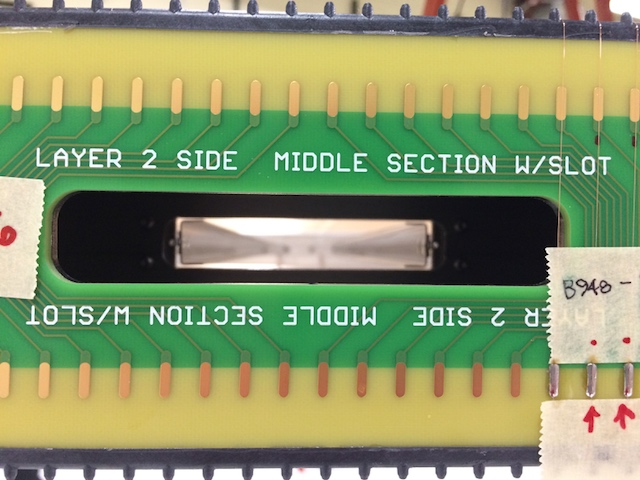
\includegraphics[height=0.3\textheight]{SideBoardSlot.jpg}}
\fbox{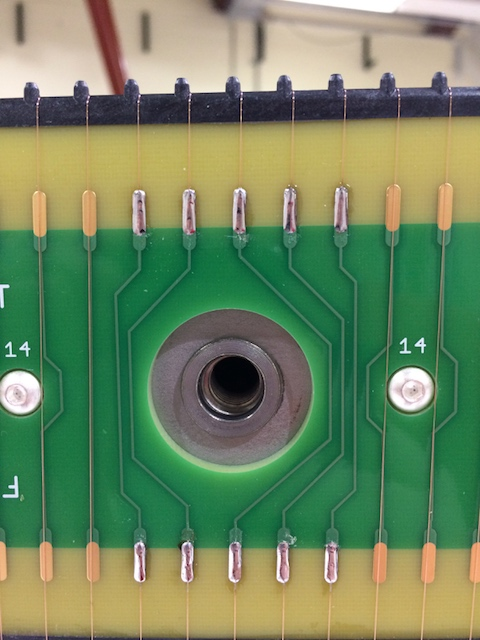
\includegraphics[height=0.3\textheight]{SideBoardRoundHole.jpg}}
\end{dunefigure}

\begin{dunefigure}[APA side board with injection molded tooth strips]{fig:tpc_apa_sideboardphoto}{Boards with injection molded tooth strips glued on.  The left shows an end board with teeth for fixing the position of the longitudinal wires.  The teeth form small notches. The right shows a side board for fixing the position of the angled wires where the wires are angled around a pin.}% (These boards are prototype test pieces and are not used in the production APAs.)}
\setlength{\fboxsep}{0pt}
\setlength{\fboxrule}{0.5pt}
\fbox{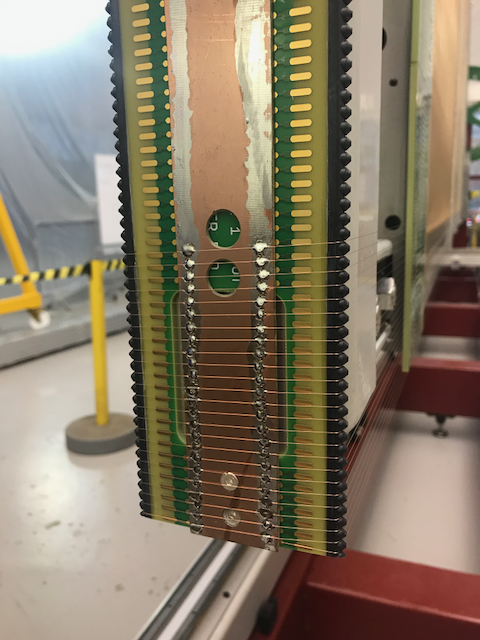
\includegraphics[height=0.3\textheight]{SacrificialBoard}}
\fbox{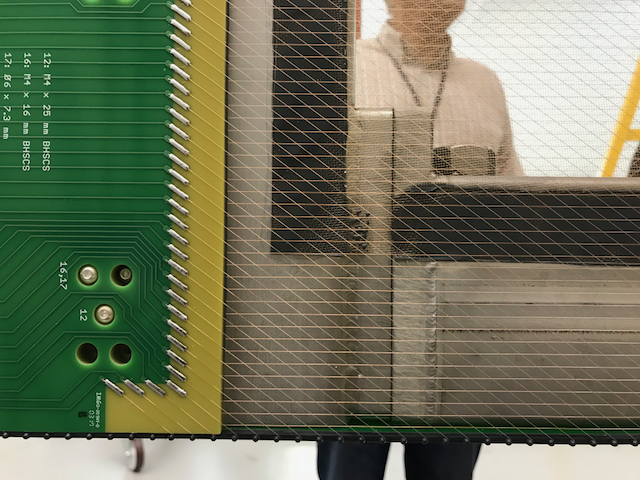
\includegraphics[height=0.3\textheight]{BoardsWithPins}}
\end{dunefigure}

The placement of the angled wires are fixed by pins as shown in the right-hand picture of Figure~\ref{fig:tpc_apa_sideboardphoto}.  The wires make a partial wrap around the pin as they change direction from the face of the APA to the edge.  The $X$- and $G$-plane wires are not pulled to the side so they cannot be pulled against a pin.  Their positions are fixed by teeth with slots, as shown in the left-hand picture in Figure~\ref{fig:tpc_apa_sideboardphoto}. 
	
The polymer used for the strips is Vectra e130i (a trade name for 30$\%$ glass filled liquid crystal polymer or LCP). It retains its strength at cryogenic temperature and has a CTE similar enough to G10 that differential contraction is not a problem.


%%%%%%%%%%%%%%%%%%%%%%%%%
\subsubsection{Support Combs}
\label{sec:combs}

Support combs are glued at four points along each side of the APA, along the four cross-beams. These combs maintain the wire and plane spacing along the length of the APA. A dedicated jig is used to install the combs and provides the alignment and the pressure to allow the glue to dry. The glue used is the Gray epoxy 2216 described below. An eight-hour cure time is required after comb installation on each side of the APA before the jig can be removed and production can continue.


%%%%%%%%%%%%%%%%%%%%%%%%%
\subsubsection{Glue and Solder}
\label{sec:glue-solder}

The ends of the wires are soldered to pads on the edges of the wire boards.  Solder provides both an electrical connection and a physical anchor to the wires. Once a wire layer is complete, the next layer of boards are glued on, this glue providing an additional physical anchor. Gray epoxy 2216 by 3M is used for the glue.  It is strong, widely used (therefore much data is available), and it retains good properties at cryogenic temperatures.  A 62$\%$ tin, 36$\%$ lead and 2$\%$ silver solder was chosen.  A eutectic mix (63/37) is the best of the straight tin/lead solders but the 2$\%$ added silver gives better creep resistance.

\begin{comment}
\subsection{Quality assurance}
Three primary quality-assurance procedures are followed during production. These are
\begin{enumerate}
\item APA-frame geometry measurements,
\item Wire-tension measurements,
\item Electrical tests on each wire layer.
\end{enumerate}

\subsubsection{APA-frame geometry}

Upon receipt of the rolled hollow section steel for the frames, a selection procedure is followed to choose the sections of the steel most suited to achieving the geometrical tolerances. This procedure is documented in document PSL-TN-2013-04.

Once an APA frame is complete, a laser survey of the back face of the frame is taken to ensure the APA satisfies the flatness criteria. The APA-frame geometry requirements are listed in table~\ref{tab:APAFrameFlatness}, and are further documented in DUNE-DocDB-1300.

\begin{dunetable}[APA-frame flatness requirements]{lc}{tab:APAFrameFlatness}{APA-frame flatness requirements. For more details see PSL-TN-2016-3.}
Criterion & Tolerance \\ \toprowrule
Overall flatness & \SI{11}{mm} \\
Overall bow & \SI{11}{mm} \\
Overall twist & \SI{2}{mm / m}\\ \colhline
Twist zone 1 & \SI{2}{mm / m}\\
Twist zone 2 & \SI{2}{mm / m}\\
Twist zone 3 & \SI{2}{mm / m}\\
Twist zone 4 & \SI{2}{mm / m}\\
Twist zone 5 & \SI{2}{mm / m}\\ \colhline
\multicolumn{2}{c}{\bf Fold --- back datum side} \\
Food tube & \SI{1.2}{mm} \\
Rib 1 & \SI{1.2}{mm} \\
Rib 2 & \SI{1.2}{mm} \\
Rib 3 & \SI{1.2}{mm} \\
Rib 4 & \SI{1.2}{mm} \\ \colhline
\multicolumn{2}{c}{\bf Fold --- front side} \\
Rib 1 & \SI{1.2}{mm} \\
Rib 2 & \SI{1.2}{mm} \\
Rib 3 & \SI{1.2}{mm} \\
Rib 4 & \SI{1.2}{mm} \\
\end{dunetable}

Once the photon-detector rails have been installed, a go-no-go device is inserted to ensure there is adequate clearance for the photon detectors. (This device is simply an oblong piece of perspex with dimensions just slightly larger than those of the photon detectors.)

\subsubsection{Wire-tension measurements}

Once each wire layer has been wound, the tension of each wire is measured, using a laser-based system. (It is hoped that an electrical system will become available in the near future.) Wire tensions are required to be in the range $3.5\textrm{--}\SI{7.5}{N}$ for wires longer than \SI{750}{mm} and in the range $2.0\textrm{--}\SI{7.5}{N}$ for wires shorter than \SI{750}{mm}.

\subsubsection{Electrical tests}

Electrical tests (leakage and isolation) are performed on each wire, once each wire layer has been wound. There must be no leakage current greater than \SI{0.5}{nA} at a \SI{1}{kV} bias. The measured current between adjacent wires, when biased at \SI{1}{kV}, must not exceed \SI{100}{nA} (corresponding to a resistance of \SI{10}{G\ohm}).
\end{comment}

